%------------------ vorlage.tex ------------------------------------------------
%
% LaTeX-Vorlage zur Erstellung von Projektdokumentationen
% im Fachbereich Informatik der Hochschule Trier
%
% Basis: Vorlage 'svmono' des Springer Verlags
% Bearbeiter: Hermann Schloß, Christian Bettinger
%
%-------------------------------------------------------------------------------


%------------------ Präambel ---------------------------------------------------
\documentclass[envcountsame,envcountchap deutsch]{i-studis}

\usepackage[utf8]{inputenc}

\usepackage[a4paper]{geometry}
\usepackage[english, ngerman]{babel}

\usepackage[pdftex]{graphicx}
\usepackage{epstopdf}

\usepackage{listings}

\usepackage[german, ruled, vlined]{algorithm2e}
\usepackage{amssymb, amsfonts, amstext, amsmath}
\usepackage{array}
\usepackage[skip=10pt]{caption}
\usepackage[usenames, dvipsnames]{color}
\usepackage[pdftex, plainpages=false]{hyperref}
\usepackage{textcomp}
\usepackage{hyperref}
\usepackage{graphicx}
\usepackage{fancyhdr}
\usepackage{algorithmic}

\usepackage{bibgerm}
\bibliographystyle{geralpha}

\usepackage{makeidx}
\usepackage{multicol}
\makeindex

\pagestyle{myheadings}
\setlength{\textheight}{1.1\textheight}
\setlength{\parindent}{0pt}

\lstset{
	language=[Sharp]C,
	basicstyle=\scriptsize\ttfamily,
	commentstyle=\scriptsize\ttfamily\color{Gray},
	identifierstyle=\scriptsize\ttfamily,
	keywordstyle=\scriptsize\ttfamily,
	stringstyle=\scriptsize\ttfamily,
	tabsize=4,
	numbers=left,
	numberstyle=\tiny,
	numberblanklines=false,
	frame=single,
	framesep=3mm,
	framexleftmargin=7mm,
	xleftmargin=10mm,
	linewidth=144mm,
	captionpos=b,
}



%------------------ Manuelle Silbentrennung ------------------------------------
%\hyphenation{Ele-men-tar-ob-jek-te ab-ge-tas-tet Aus-wer-tung House-holder-Matrix Least-Squares-Al-go-ri-th-men}


%------------------ Titelseite -------------------------------------------------
\begin{document}
\begin{center}
	{\Huge\bfseries Business Plan für} \\
	{\Huge\bfseries Dungeon Rat Games} \\
	
\end{center}

\begin{figure}[h]
	\centering
	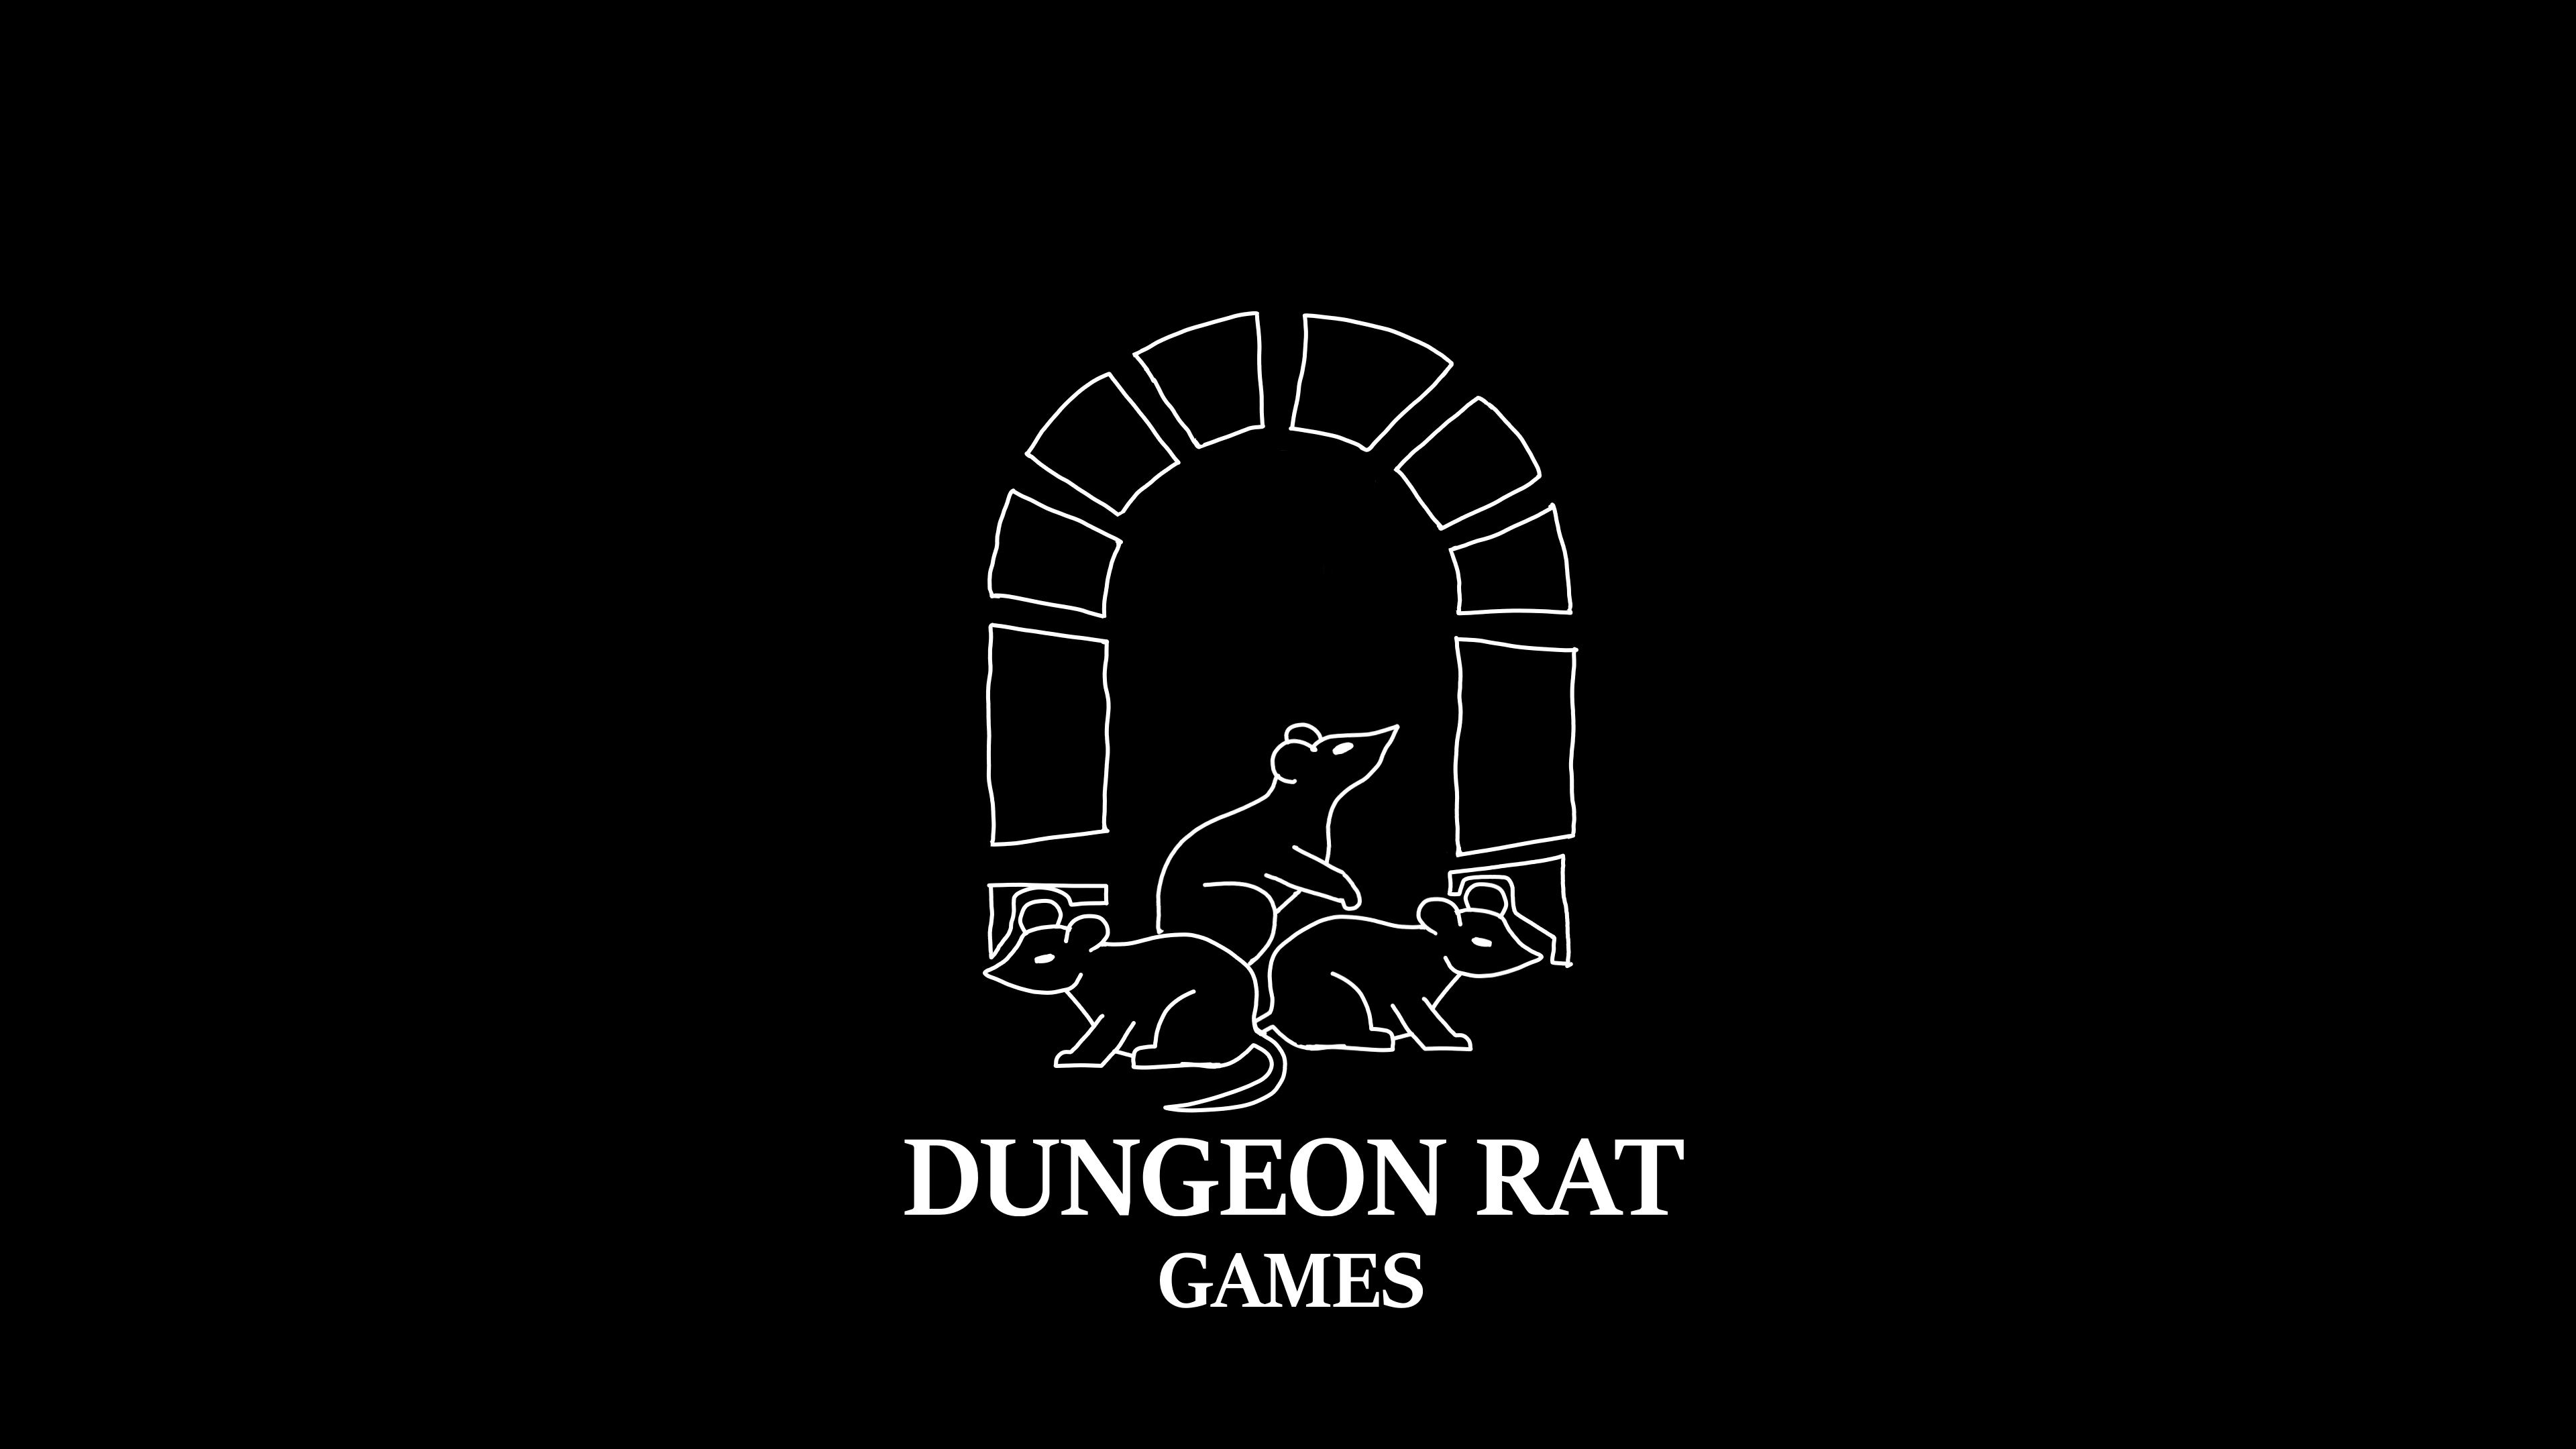
\includegraphics[width=1\textwidth]{images/DungeonRatGamesIcon.png}
	\label{fig:meinbild}
\end{figure}

\pagenumbering{arabic}
%------------------ Vorwort, Kurzfassung, Verzeichnisse ------------------------

%\kurzfassung
%Eine Kurzfassung

\tableofcontents										% Inhaltsverzeichnis
%\listoffigures
%\lstlistoflistings

% Du musst nicht alles beschreiben aber du kannst :) Neues Game yey
%------------------ Kapitel ----------------------------------------------------

\chapter{Executive Summary}
Dungeon Rat Games ist ein Indie-Spieleentwichlungs Unternehmen dessen Sitz im Saarland ist. Dabei wird sich auf das Entwickeln von Adventure Fantasy-Rollenspiele sowie Spiele mit außergewöhnlichen Mechaniken spezialisiert.
\\
\\
Es wird sich auf die Entwicklung von Hochwertigen PC-Rollenspielen mit einer ausgeprägten Atmosphäre,anspruchsvollen Spielmechaniken, erzählerischer Tiefe sowie Wiederspielwert konzentriert.
\\
\\
Die Spiele werden mit Hilfe der Unity-Engine entwickelt und die Veröffentlichung wird zunächst digital über Plattformen wie Steam oder Itch.io erfolgen.
\\
\\
Das Unternehmen wurde als Einzelunternehmen gegründet wobei der Gründer die Geschäftsführung sowie die kreativen, technischen und organisatorische Aufgaben übernimmt. Falls es spezielle Aufgaben gibt werden externe Dienstleister beauftragt welche bevorzugt aus dem Saarland oder der näheren Umgebung kommen.
\\
\\
Das erste Entwicklungsprojekt ist ein eigenständig entwickeltes First-Person-Dungeon-Crawler  Rollenspiel das als Grundlage für den langfristigen Aufbau einer eigenen Spielmarke dienen soll.
\\
\\
Die Finanzierung soll durch eine Kombination aus Eigenkapital und öffentlichen Fördermitteln erfolgen.
\\
\\
Das langfristige Ziel besteht darin, Dungeon Rat Games als wirtschaftlich tragfähiges Indie-Entwicklerstudio im Saarland zu etablieren und ein nachhaltiges Portfolio an Spielen aufzubauen.

\chapter{Unternehmensbeschreibung}
\section{Unternehmensprofil}
Name des Unternehmens : Dungeon Rat Games \\
Geschäftstätigkeit : Entwicklung und Vermarktung eigener Computerspiele \\
Branche : Digitale Spieleentwicklung \\
Unternehmensstandort: Saarland, Deutschland \\
Unternehmensform: Einzelunternehmen \\
Inhaber: Philip Borngässer \\
\\
Durch die schlanke Unternehmensstruktur und die Nutzung digitaler Entwicklungsprozesse sollen die laufenden Kosten gering gehalten werden.
\section{Unternehmensmission}
Die Mission von Dungeon Rat Games ist die Entwicklung von möglichst immersiven Spielen die Spieler durch ihre Atmosphäre, Geschichte und Entscheidungsfreiheit begeistern.\\
Dabei soll nicht die Spieldauer des Spiels überzeugen sondern die Qualität und die Immersion des Produktes. 

\section{Unternehmensvision}
Langfristig soll sich Dungeon Rat Games im umkämpften Videospielmarkt  als Indie Entwickler etablieren. Zusätzlich soll eine eigene Marke sowie Community aufgebaut werden ,die im deutschen und internationalen Markt präsent ist.
\\
\\
Das Unternehmen sieht einen schrittweise Aufbau des Studios mit zusätzlichen Mitarbeitern vor.
\section{Rechtsform}
Die Gründung erfolgt zunächst als Einzelunternehmen.\\
Dadurch wird ein kostengünstiger Einstieg ermöglicht.\\
Falls externe Eigenkapitalinvestoren beteiligt werden, soll die Rechtsform zu einer UG oder GmbH umgewandelt werden.

\chapter{Geschäftsidee und Leistungsangebot}
\section{Geschäftskonzept}
Das Kerngeschäft besteht in der eigenständigen Entwicklung und Vermarktung von Videospielen.\\
Die Aufgaben des Unternehmens sind:\\
\\
Konzeption und Testen von Spielideen. \\
Entwicklung von Welten und Geschichten von Fantasy Welten. \\
Umsetzung von Spielideen in Unity3D.\\
Erstellung von Assets für Videospiele. \\
Qualitätssicherung und Fehlerbehebung. \\
Marketing sowie Community Aufbau. \\
Veröffentlichung und langfristige Betreuung von Produkten. \\
Erstellung von Erweiterungen für Videospielen. \\

\section{Geplante Produkte}
Zunächst wird der First-Person-Dungeon-Crawler „Thorned King“ entwickelt.
\subsection{Spielidentität von Thorned King}
„Thorned King“ ist ein First-Person-Dungeon-Crawler, dessen Spielfortschritt auf dem Wissen des Spielers
über die Welt basiert. Dabei kämpft sich der Spieler als Abenteurer durch ein dornenüberwuchertes Schloss und deckt so nach und nach dessen Geheimnisse auf.

\pagebreak
\section{Technische Grundlage}
Entwickelt wird zunächst mit Unity3D.\\
Das Erstellen von 3D Assets erfolgt mit Blender. \\
Für die Versionskontrolle wird auf Git zurückgegriffen.
\section{Einnahmequellen}
Die Einnahmequellen beschränken sich zunächst auf das Entwickeln und Verkaufen von Spielen.\\
Nach dem Veröffentlichen des ersten Spiels sollen durch bezahlbare Erweiterungen zusätzliche Einnahmen generiert werden.


\chapter{Markt- und Wettbewerbsanalyse}
\section{Marktumfeld}

Der internationale Videospielmarkt bietet Indie Entwicklern die Möglichkeit eigene Produkte weltweit anzubieten.
\\
\\
Darüber hinaus bieten Digitale Plattformen die Möglichkeit ohne eigene Infrastruktur international Kunden zu erreichen.
\\
\\
Der Rollenspiel Markt wird durch etablierte Studios und eine große Zahl unabhängiger Entwickler geprägt.
\\
Dungeon Rat Games positioniert sich nicht als direkte Konkurrenz zu großen AAA Produktionen sondern als spezialisiertes Indie Studio das Wert auf Qualität statt auf eine hohe Spielzeit  und viel Inhalt legt.

\section{Zielgruppe}
Die primäre Zielgruppe umfasst Spieler mit Interesse an: \\
\\
Rollenspielen.\\
Kurzen Spielen mit einer tiefen Geschichte. \\
Etwas schwereren Spielen. \\
Ungewöhnlichen Spielmechaniken.\\

Die Vermarktung erfolgt international, wobei Deutschland im Vordergrund steht da gerade Rollenspiele und Spiele mit Tiefer Geschichte wie Point-And-Click Spiele sehr beliebt sind. 
\pagebreak
\section{Wettbewerbsumfeld}
Als relevante Marktteilnehmer und qualitative Vergleichsprodukte gelten : \\
\\
Larian Studios. \\
From Software. \\
Warhorse Studios. \\
Andere Indie Entwickler ,deren Schwerpunkt Adventure und Rollenspiele sind.
\\
\\
Die genannten Unternehmen dienen als Orientierung hinsichtlich Qualität und potentiellen Märkten.

\section{Wettbewerbsvorteile}
Das Unternehmen hat folgende Wettbewerbsvorteile :\\
\\
Community Nähe durch kleines Unternehmen.\\
Klare Spezialisierung auf Rollenspiele. \\
Konzentrieren auf eine starke Spielerfahrung um Kunden an das Unternehmen zu binden. \\
Schlanke Produktionsstruktur. \\
Aufbau einer Marke und Nutzungsrechten.\\

\chapter{Marketing- und Vertriebsstrategie}
\section{Vertriebsplattform}

Der Hauptvertrieb erfolgt über Steam.\\
Weitere Plattformen werden nach der Veröffentlichung geprüft\\

Weitere Plattformen sind :\\
GOG.com \\
itch.io \\
Epic Games Store \\
Später gegebenfalls eine Konsolenplattform.\\
\\
Dies erfolgt nur wenn sich das Vorhaben wirtschaftlich lohnt.
\pagebreak
\section{Marketing Strategie}

Das Marketing beginnt bereits während der Entwicklung.\\
Dabei ist das Ziel ,eine Community aufzubauen die das Interesse am ersten Produkt sowie die möglichen Einnahmen durch Wishlists bei Veröffentlichung messbar macht.

\subsection{Youtube}
Kurze Devlogs mit hoher Qualität \\
Gameplay Trailer \\
Shorts um unterhaltsame Momente in der Entwicklung festzuhalten\\
\subsection{Discord}
Aufbau einer Community \\
Direktes Feedback zu Spielmechaniken \\
Potentielle Playtester \\
\subsection{TikTok und Instagram}
Erneutes hochladen des Shortform Contents \\
Conzept Art \\

\subsection{Steam}
Veröffentlichen einer Demo \\
Updates \\
Regelmäßige Neuigkeiten \\
\subsection{Presse und Content Creator}

Kontaktaufnahem mit Streamern
\\ Kontakaufnahme mit Rollenspiel Youtubern vorallem im deutschen Raum.
\\ Bereitstellen von Testversionen
\section{Marketing Ziele}
 Vor der Veröffentlichung soll eine aktive Community, eine aussagekräftige Steam-Präsenz und eine ausreichende Anzahl an Wunschlisten aufgebaut werden. 
 


\chapter{Unternehmensorganisation und Personalplanung}
\section{Unternehmensführung}
Das Unternehmen wird zunächst vom Inhaber in Vollzeit geführt.
\section{Externe Dienstleistungen}
Zur Sicherung der Produktqualität werden bei Bedarf externe Spezialisten eingesetzt.\\
Dazu zählen insbesondere : \\
2D und 3D Artists. \\
QA Tester. \\
\section{Personalentwicklung}
Nach erfolgreicher Gründungsphase und dem Nachweis der Tragfähigkeit des Geschäftsmodells kann das Unternehmen schrittweise wachsen.
\\
Die erste Personelle Erweiterung könnte durch einen Artist oder Game Designer erfolgen.

\chapter{Zeitplanung}
\begin{table}[ht]
	\centering
	\begin{tabular}{|p{5cm}|l|p{9cm}|}
		\hline
	 \textbf{Phase}  & \textbf{Zeitraum}& \textbf{Ergebnis} \\ \hline
	 Vorproduktion  & 4 Monate& Erste Mechaniken sind implementiert \\ \hline
	 Prototyp  & 12 Monate& Spielbarer Kern des Spiels und Förderanschluss \\ \hline
	 Prototyp  & 15 Monate& Vorzeigbare Demo \\ \hline
	 Produktionsplanung  & 17 Monate& Produktionsplanung \\ \hline
	 Hauptproduktion  & 22 Monate& Entwicklung des vollen Spiels \\ \hline
	 Qualitätssicherung  & 24 Monate& Polish \\ \hline
	 Veröffentlichung  & 26 Monate& Realese \\ \hline
	 Updates  & 26 Monate& Realese Begleitung und Updates \\ \hline
	\end{tabular}
\end{table}

Der Zeitplan setzt eine rechtzeitige Finanzierung voraus.\\
Die Prototypen Phase wurde durch die Beantragung der Games-Förderung im Saarland gesondert geplant.
(Siehe Anhang)
\chapter{ Investitions- und Kapitalbedarfsplanung}
\section{Vorhandenes Eigenkapital}
Der Gründer verfügt über ein Startkapital von knapp 15.000€ \\
Dieses Kapital dient als Mitfinanzierung des Entwicklungsprozesses und der Sicherung einer finanziellen Reserve.

\section{Projektbezogenes Entwicklungsbudget des Prototypen}
Personalkosten : 48.480€\\
Software : 965€\\
Marketing : 1000€ \\
Sonstige Kosten : 600€ \\
Gesamt : 51.045 €\\
\\
Genauere Angaben findet man im Kosten und Finanzierungsplans des Prototypen. (Siehe Anhang)
\chapter{Finanzierungsstrategie und Fördermittel}
Die Finanzierungsstrategie bezieht sich auf das erste Jahr. Daraufhin wird sich um weitere Fördermittel bemüht.
\section{Eigenkapitalfinanzierung}
Der Gründer bringt 15.000€ Eigenkapital mit. \\
Dieses Kapital dient vor allem zur : \\
Mitfinanzierung der Entwicklung. \\ \\
Anschaffung technischer Ausstattung. \\
Darstellung des eigenen Engagements.
\section{Games-Förderung Saarland}
Die Games-Förderung Saarland bietet die Möglichkeit für junge Unternehmen an zusätzliches Kapital zu gelangen. \\
Diese Förderung wurde beantragt und deckt knapp 75\% des benötigten Kapitals ab. 
\section{Modellrechnung zur saarländischen Förderung}

\begin{table}[ht]
	\centering
	\begin{tabular}{|p{6cm}|p{3cm}|}
		\hline
		\textbf{Finanzierungsbestandteil}  &\textbf{Betrag} \\ \hline
		Benötigtes Kapital  & 51.045,00 € \\ \hline
		Fördermittel  & 34.740,00 €\\ \hline
		Eigenanteil  & 12.761,25 € \\ \hline
	\end{tabular}
\end{table}

Die Rechnung stellt einen möglichen Förderfall dar für das erste Jahr des Unternehmens.

\section{Bundesweite Games-Förderung}
Für eine Bundesförderung wird eine Kapitalgesellschaft benötigt. Daher entfällt diese Möglichkeit zunächst ,bis das Unternehmen gewachsen ist und zu einer GmbH umgewandelt wird.
\section{Weitere Finanzierungsmöglichkeiten}
Weitere Finanzierungsmöglichkeiten wären: \\\\
Eine Partnerschaft mit einem Publisher. \\
Crowdfunding. \\
Nebentätigkeiten für andere Unternehmen. \\
\chapter{Umsatz- und Rentabilitätsplanung}
\section{Preisgestaltung}
Für das erste Spiel wird beispielsweise ein Preis von knapp 20€ verlangt.\\
\\
In der Umsatzkalkulation muss die Umsatzsteuer und die Beteiligung der Vertriebsplattform berücksichtigt werden. Nach Abzügen erhält man knapp 11,76€ Netto pro Exemplar.
\\
\\
Der tatsächliche Erlös ist schwer zu berechnen durch Rabatte, \\Rückerstattungen, regionale Preise sowie verschiedene Plattformkonditionen.
Da die ersten 2 Jahre kein Geld eingenommen wird müssen Potentiell 2 Förderperioden berücksichtigt werden. Dafür wird der doppelte Wert der ersten Periode genommen um den benötigten Umsatz zu berechnen. In diesem Fall 102.090€.
Somit müssen knapp 10000 Einheiten verkauft werden damit das Unternehmen rentabel wird.

\section{Absatzplanung}
\begin{table}[ht]
	\centering
	\begin{tabular}{|p{3cm}|p{3cm}|}
		\hline
		\textbf{Geschäftsjahr}  & \textbf{Geplante Verkäufe} \\ \hline
		Jahr 1  & 0 \\ \hline
		Jahr 2  & 3000 \\ \hline
		Jahr 3  & 2500 \\ \hline
		Jahr 4  & 2000 \\ \hline
		Jahr 5  & 2000 \\ \hline
		Jahr 6  & usw. \\ \hline
	\end{tabular}
\end{table}

In der regel dauert es mehrere Jahre in Kombination mit Updates und Sales um das ausgegebene Kapital zu generieren. Es ist wichtig ,dass während dieser Zeit den Kontakt zur Community erhalten und die Einnamen in die Entwicklung neuer Projekte zu stecken.

\section{Umsatzplanung}
Die Verkaufsprognose muss durch Demo-Feedback, Wunschlisten sowie Marketingreichweite überprüft werden. 
\\
\\
Der Umsatz wird über mehrere Jahre generiert. Es wird davon ausgegangen das knapp 30000€ im ersten Jahr des Verkauft eingenommen wird. Realistisch gesehen ist der Break-Even Point nach 4 Jahren Verkauf erreicht.
\section{Betriebskostenplanung}
Dies entspricht den ersten 3 Jahren Entwicklung.
Da der Inhaber auch der Entwickler des Spiels ist fließen die Lebenshaltungskosten kosten in die Betriebskostenplanung.
\begin{table}[ht]
	\centering
	\begin{tabular}{|p{5cm}|p{3cm}|p{3cm}|p{3cm}|}
		\hline
		\textbf{Kostenposition}  & \textbf{Jahr 1} & \textbf{Jahr 2} & \textbf{Jahr 3}\\ \hline
		Personalkosten  & 48.480,00 €& 48.480,00 €& 48.480,00 € \\ \hline
		Marketing & 1000€ & 1300€ & 1300€ \\ \hline
		Sonstige Kosten & 600€ & 600€ & 600€ \\ \hline
		Hard und Software  &965€ & 0€ & 0€ \\ \hline
		Gesamt  &51.045,00 € &51.045,00 € & 51.045,00 € \\ \hline
	\end{tabular}
\end{table}

Die Kostenplanung ist eine einfache Rechnung und orientiert sich hierbei an dem ersten Jahr der Entwicklung.


\section{Vereinfachte Ergebnisprognose}

\begin{table}[ht]
	\centering
	\begin{tabular}{|p{5cm}|p{3cm}|p{3cm}|p{3cm}|}
		\hline
		\textbf{Geschäftsjahr}  & \textbf{Erlös}  &\textbf{ Betriebskosten} & \textbf{Ergebnis}\\ \hline
		Jahr 1  & 0 €& 51.045,00 €& -51.045,00 € \\ \hline
		Jahr 2 & 30000€ & 51.045,00€ & -72.090€ \\ \hline
		Jahr 3  & 30000€ & 51.045,00€ &-90.090€ \\ \hline
	\end{tabular}
\end{table}

Diese Planung verdeutlicht, dass trotz erfolgreicher Prototypen Förderung eine zusätzliche Finanzierung der Hauptproduktion erforderlich ist.

\chapter{Liquiditätsplanung und Kapitalabsicherung}

Die Entwicklung eines Videospiels verursacht zunächst Kosten, während die wesentlichen Verkaufserlöse erst nach der Veröffentlichung entstehen.
\\
\\
Dabei ist auf folgendes zu achten :\\
Entwicklung und klares trennen von Projektphasen.\\
Regelmäßige Überprüfung von Ausgaben.\\
Nutzung öffentlicher Fördermittel.\\
Frühzeitige Vorbereitung der Anschlussfinanzierung.\\
Vermeidung unnötiger Fixkosten durch z.B Abos.\\

Vorfinanzierung und Eigenanteil müssen abgesichert sein.\\

\chapter{Chancen- und Risikoanalyse}
\section{Chancen}
Die kleine Unternehmensstruktur führt zu reduzierten Personal und Raumkosten.\\\\

Ein erfolgreiches Spiel ermöglicht es durch Zusatzinhalte mit wenig Aufwand zusätzliche Einnahmen zu generieren und langfristig eine Community aufzubauen.\\\\

Das Saarland verfügt über spezielle Förderprogramme um Unternehmen die sich auf das Entwickeln von Videospielen konzentrieren zu unterstützen. \\\\

Digitale Vertriebsplattformen ermöglichen eine weltweite Vermarktung und Veröffentlichung.\\\\

Die Spezialisierung auf Rollenspiele mit einem Schwerpunkt auf Geschichte ermöglicht es, gerade in Deutschland, eine feste und starke Community aufzubauen. \\\\

Für Adventure und Rollenspiele kann in der Regel mehr Geld verlangt werden ,als für andere Spiele Genres.

\pagebreak
\section{Risiken}
\begin{table}[ht]
	\centering
	\begin{tabular}{|p{5cm}|p{8cm}|p{3cm}|p{3cm}|}
		\hline
		\textbf{Risiken}  & \textbf{Gegenmaßnahme}  \\ \hline
		Zu lange Entwicklungszeit  & Verringerung des Spielumfangs  \\ \hline
		Geringe Verkaufszahlen & möglichst früher Aufbau einer Community  \\ \hline
		Starke Konkurrenz  & Abheben durch Besondere Mechaniken\\ \hline
		Keine Förderung  & Andere Finanzierungsmöglichkeiten \\ \hline
		Technische Probleme  & Regelmäßige Builds und Tests\\ \hline
		Kein Spielspaß  & Regelmäßige Playtests\\ \hline
		Abhängigkeit zu Steam  & Ausbreiten zu anderen Vermittlungsplattformen\\ \hline
		Zu hohe Kosten  & Regelmäßige Kostenkrontrolle\\ \hline
		Liquiditätsprobleme  & Rücklagen und Anschlussfinanzierungen\\ \hline
	\end{tabular}
\end{table}

\section{Risikobegrenzung}

Das erste Projekt wird bewusst als übersichtliches Rollenspiel konzipiert.\\
Dabei stehen besondere spielerische Mechaniken und die Geschichte im Vordergrund.\\
\\
Es wird auf typische Fallhürden wie eine Synchronisation, eine riesige \\ Open World, sowie
komplexe Systeme bewusst verzichtet, um Kosten und Risiken gering zu halten.

\chapter{Unternehmensentwicklung und Wachstumsstrategie}
\section{Gründung und Prototyp: 1 Jahr}
Gründung von Dungeon Rat Games.\\
Aufbau von Infrastruktur.\\
Aufbau einer Community.\\
Beantragung der Prototypen Förderung im Saarland.\\
Entwicklung eines spielbaren Prototypens.\\
\section{Hauptproduktion und erster Release : 2 Jahr}
Beantragung der Gamesförderung im Saarland.\\
Weiterenwicklung des Prototypens in eine Demo und dann in ein fertiges Spiel.\\
Aufbau der Steam Präsenz.\\
Vorbereitung und Veröffentlichung des Spiels.\\
Konzeptfindung weiterer Spielideen für das Folgejahr.\\
Erste Einnahmen.\\
\section{Markenausbau : Jahr 3}
Beantragung der Prototypenförderung im Saarland.\\
Erweiterung des veröffentlichten Spiels.\\
Veröffentlichen des ersten Spiels auf anderen Plattformen.\\
Entwicklung zusätzlicher Inhalte.\\
Ausbau eines weiteren Rollenspiel Prototypen.\\

Das Unternehmen soll langfristig ein Portfolio von Spielen aufbauen und sich so nach und nach von einem Inhaber geführten Einzelunternehmen zu einer UG oder GmbH mit mehreren Mitarbeitern entwickeln.

\chapter{ Investoren- und Finanzierungskonzept}
\section{Finanzierungsbedarf}
In der ersten Finanzierungsphase wird ein Projektvolumen von 51.045€ angesetzt.\\
Dabei sind 11.580,00 € Eigenanteil (25\%) und 34.740,00 € (75\%) Fördermittel.
\section{Perspektivische Anschlussfinanzierung}
Nach Fertigstellung des Prototypens soll eine weitere Finanzierung für die Hauptproduktion angestrebt werden.\\\\
Finanzierungsmöglichkeiten sind : \\
Publisher. \\
Investoren. \\
Fördermittelgeber. \\
\\
Nach der Produktion des Prototypens wird der tatsächliche Produktionsaufwand und der Finanzierungsaufwand ermittelt.

%------------------ Literaturverzeichnis & Index -------------------------------
%\bibliography{Referenzen}



%------------------ Anhänge ----------------------------------------------------
\begin{appendix}
	%\chapter{Selbstständigkeitserklärung}

\begin{description}

\item[$\Box$] Diese Arbeit habe ich selbstständig verfasst und keine anderen als die angegebenen Quellen und Hilfsmittel verwendet.\\

\item[$\Box$] Diese Arbeit wurde als Gruppenarbeit angefertigt. Meinen Anteil habe ich selbstständig verfasst und keine anderen als die angegebenen Quellen und Hilfsmittel verwendet.\\

Namen der Mitverfasser:
\vspace{3cm}

Meine eigene Leistung ist:
\vspace{3cm}

\end{description}

\vspace{3cm}

\begin{minipage}[t]{3cm}
	\rule{3cm}{0.5pt}
	Datum
\end{minipage}
\hfill
\begin{minipage}[t]{9cm}
	\rule{9cm}{0.5pt}
	Unterschrift der Kandidatin/des Kandidaten
\end{minipage}
	% Selbstständigkeitserklärung
\end{appendix}


\end{document}
